\documentclass[a4paper]{article}

\usepackage{graphicx}

\usepackage{vmargin}
  \setpapersize{A4}
  \setmargins{2cm}{2cm}% % linker & oberer Rand
             {17.5cm}{24cm}%   % Textbreite und -h�he
             {12pt}{25pt}%   % Kopfzeilenh�he und -abstand
             {0pt}{30pt}%    % \footheight (egal) und Fu�zeilenabstand

\begin{document}

\title{The Palladio Component Model}
\author{Steffen Becker}
\maketitle

\vspace{3cm}
\tableofcontents

\newpage


\section{Overview}
The Palladio component model is the meta-model for specifying component models in the context of the Palladio framework. Currently the specification of a logical view on basic components, components built by assembling components and component connections is supported. To gain a better understanding of the model take a closer look at figure \ref{fig:componentmodel}.

\begin{figure}[htb]
	\centering
		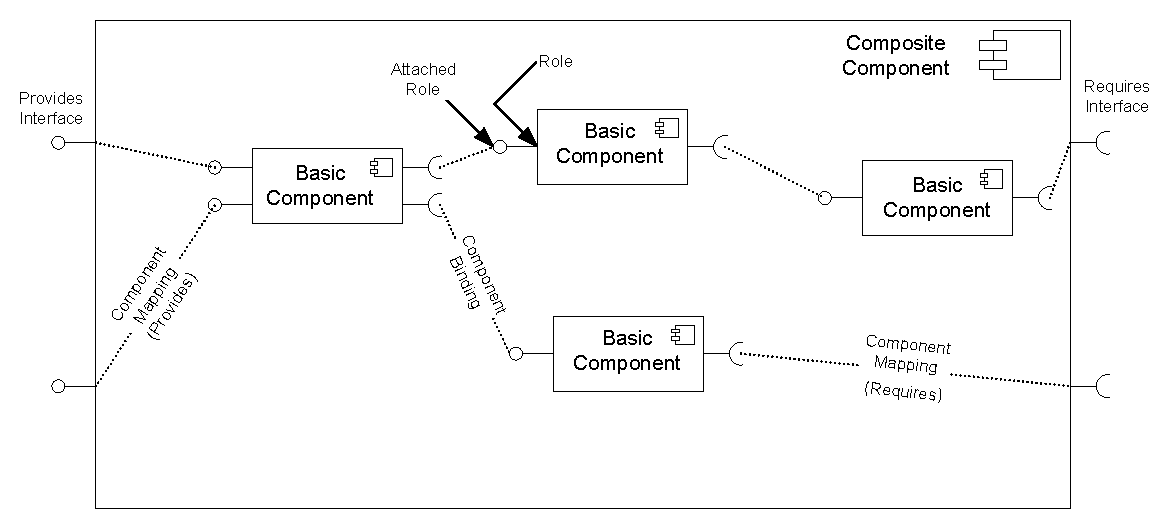
\includegraphics[scale=0.7]{pics/componentmodel.eps}
	\caption{Building blocks of the Palladio component model}
	\label{fig:componentmodel}
\end{figure}

\subsection{Components}
As depicted a component can be of two different types. 
\begin{itemize}
\item \emph{Basic Component}: A basic component can be seen as a black box entity for the component based system. There is no additional knowledge of the internal structure of those components, e.g. whether they are build from other components or not. A basic component is characterized by its interfaces as described later on.
\item \emph{Composite Component}: A composite component is a container for other components (basic or composite). It is supposed to offer a set of interfaces belonging together, e.g., by fullfiling a complete domain task. The components which are part of a composite component are wired internally by so called connections which again are introduced later.
\end{itemize}

\subsection{Roles and Interfaces}
A component has a two sets of interfaces. A set of provides interfaces, where the services the component offers to the environment are located, and a set of requires interfaces, containing all the services needed from the environment in order to operate correctly. In order to identify a single service uniquely an interface being part of a component is called a role and given a role identifier. For example, imagine a service called aService offered by two provides interfaces of the component. The first interface has the role identifier A and the second one B. Then it becomes possible to identify those services by writing A.aService and B.aService. The term "Role" comes from the role the component plays in an interaction with its environment when referring to single service calls.

An interface is described by a so called \emph{interface model}. The interface model is a container for the information that can be associated to the interface. As a minimum requirement the interface model always consists of a list of signatures stating the provides- or required services respectively. Additionally, any kind of \emph{auxiliary information} can be attached to an interface, like protocol information using FSMs or petri-nets. Other possible information can be thread safety specifications, logical constraints (pre- and postconditions) or even domain related QoS aspects. The actually needed auxiliary information is depending on the analysis one wishes to perform on the specified model.

\subsection{Connections}
The basic components and their interfaces are inter-connected in a composite component by two different types of connections.

\begin{itemize}
\item \emph{Binding}: This kind of connection is used to connect a requires interface of one component to the provides service of another component. Such a connection has the meaning that any call of the requiring component to the respective requires role is actually redirected to a call of an appropriate provided service on the providing component. Note that there might be some kind of connector involved in this process, like using a RMI or .NET Remoting call.
\item \emph{Mapping}: Mappings on the other hand are logical constructs which map the provided or required services of the composite component to contained basic components. There are two types of mappings: Provides mappings are used to map provides services to components offering those services and requires mappings are used to map required services to requires interfaces of the composite component.
\end{itemize}

The different types of connections can be seen in figure \ref{fig:componentmodel} and figure \ref{fig:connections} respectively.

\begin{figure}[htb]
	\centering
		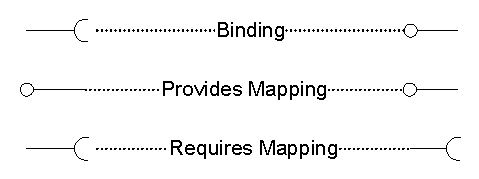
\includegraphics{pics/connections.eps}
	\caption{Different types of conncetions}
	\label{fig:connections}
\end{figure}

Note, that if you image an additional requires or provides interface respectively for the mappings then a (general) connection can be seen as a link between a requires and a provides role.

\subsection{Service Effect Specification}
The Palladio component model supports the specification of so called \emph{service effect specifications}. A service effect specification is a description of the behaviour of a single service - restricted to external interaction, i.e., if service A calls service B and C then B and C are part of the service effect specification of service A. As a service effect specification can have as many different information as an interface model, the service effect can be seen as a special kind of interface model.

The main difference between an interface and a service effect specification is the type of the signatures used in the specification. With respect to the service effect specification a role identifier needs to be added to a signature to identify the external services uniquely, e.g., consider a service calling "save" on a file and on a database simultaneously. Then, in order to differentiate both of them the role identifier like "DatabaseStore" and "FileStore" are needed. This difference is not needed for interface specifications, as a signature is already identified by the interface offering the respective service.

An example of a service effect specification consisting of the external signatures and their calling order specified as FSM is depicted in figure \ref{fig:serviceeffect}.

\begin{figure}[htb]
	\centering
		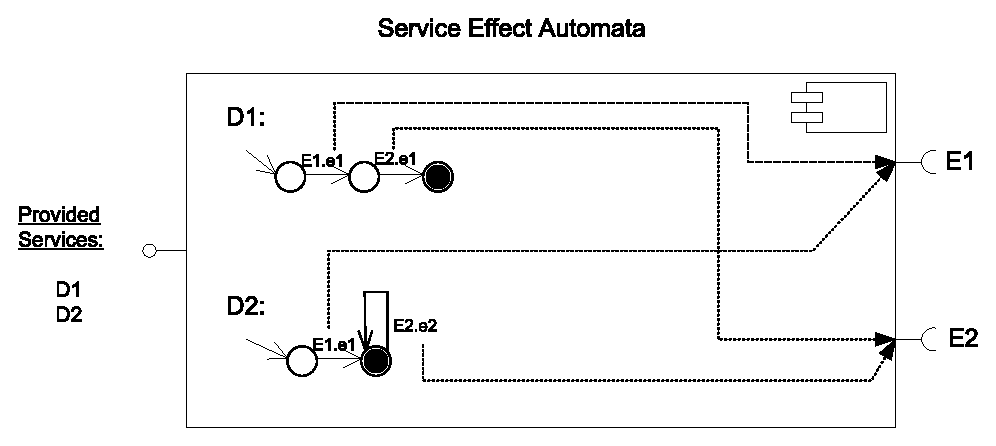
\includegraphics{pics/serviceeffect.eps}
	\caption{Example service effect specification}
	\label{fig:serviceeffect}
\end{figure}

\newpage

\section{Static Structure}
The meta-model as described in the previous section is realised in a .NET assembly. The complete structure of the interfaces involved can be seen in figure \ref{fig:classdiagramm}.

\subsection{Components}

A central interface used here as entry point for the description is IComponent and its associates IBasicComponent and ICompositeComponent.

As one of the elementary concepts of component based software engineering is the compositionality of components, e.g., to build new applications and components from existing ones, the Palladio component model supports this by the composite design pattern. The relevant part of the class digram is shown in figure \ref{fig:compositecomponent}.

\begin{figure}[!ht]
	\centering
		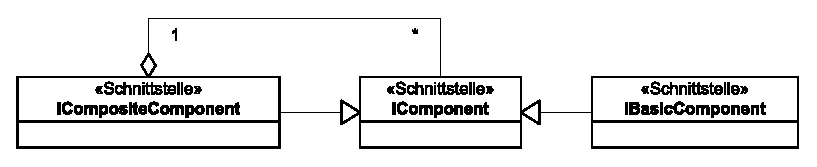
\includegraphics{pics/compositecomponent.eps}
	\caption{The composite structure of the component model}
	\label{fig:compositecomponent}
\end{figure}

The abstraction of a basic and a composite component is the IComponet interface. Common to all components is their external representation. Therefore the IComponent interface supports editing a components provides and requires roles. The internal representation of a basic and a composite component are too different so that this aspect could not be added to the IComponent interface. 

Composite components consist of a non-empty set of IComponents which make up the composite component. In addition a composite component is responsible for managing the connections (provides-, requires-mappings and bindings) of the components.

Basic components are those components that can not be split any further in components either because they don't use other components or the internal structure is simply unknown. As these components can not be decomposed further it makes sense to associate service effect specifications to basic components. The reason for attaching service effect specifications to basic components and not to single interface specifications is that we don't want to restrict the implementer of a certain provides interface to an associated service effect. The amount of external dependencies a component has to its environment is part of the design decision when implementing a single basic component.

A basic component is therefore able to map a role identifier and a signature contained in this role to a service effect specification. The mapping is a 1 to 0..1 relationship as a service effect specification is \emph{optional}. Note that if an algorithm needs a certain kind of service effect specification it should assert first, that all the required information are specified!

\subsection{Interfaces}
\begin{figure}[htb]
	\centering
		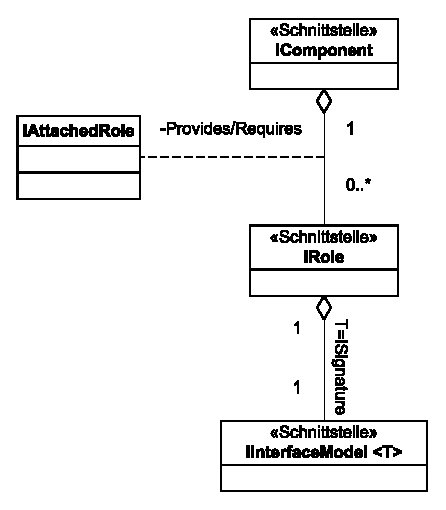
\includegraphics[scale=0.7]{pics/compinterface.eps}
	\caption{Components, Interface Models and Roles}
	\label{fig:compinterface}
\end{figure}

Associated to each component are two sets of roles: a set of provided roles and a set of required roles (see figure \ref{fig:compinterface}). The set of provided roles should have at least one element for being a valid component. Each role introduces an identifier unique to the component and has exactly one interface model associated to it (see below for a description of those). Important is that the association between a component and its role respectively the identifier of the role is a \emph{named} association called IAttachedRole which is used in an IConnection.

\subsection{Interface Model}
An important concept in the Palladio component model is the one of \emph{interface models} (see figure \ref{fig:intefacemodel}).

\begin{figure}[htb]
	\centering
		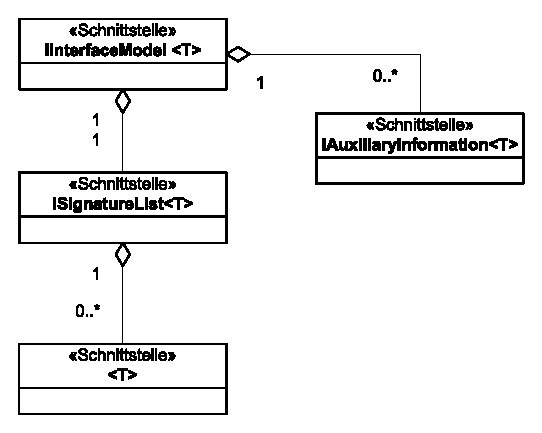
\includegraphics[scale=0.6]{pics/intefacemodel.eps}
	\caption{Interface Model}
	\label{fig:intefacemodel}
\end{figure}

An interface model is used to abstract away from the different approaches to specify rich interfaces. Rich interfaces are those having more information than only a list  of signatures of the services of the respective interface. Additional, or like it is called here, auxiliary information can contain protocol specifications, i.e., protocol FSMs, petri-nets, pre- and postconditions, re-entrance specifications, QML contracts, ... As today's component technologies only support signature list based provides interface specifications only the signature list is mandatory. Any other (more or less scientific) auxiliary specification data can be attached according to the algorithms needed in a specific context. 

There is a resulting problem with this concept. For the auxiliary information it might be important to check the consistency of the specification data. But the consistency depends on the checking if the signatures in the auxiliary specification are part of the signatures contained in the signature list. Therefore the component model uses an observer pattern on the signature list to inform the auxiliary specification objects about changes on it. The FSM protocol auxiliary specification uses this concept for example to automatically adjust the FSM's input alphabet to be identically to the signatures in the signature list. The observer pattern is implemented by using the .NET event mechanism, the necessary delegates can be found in the main namespace. As the usage of this concept can't be enforced by the type system, please read the respective code documentation before creating a new auxiliary specification object.

An other important concept is the usage of a \emph{generic} interface model. The generic type parameter is a place holder for the type of the signature contained in the signature list. As described in the introduction there are two types of signatures: internal signatures which are part of a certain interface and external signature referencing services outside of the containing component. The problem with this idea is that support for generic data types is initially introduced in C\# 2.0 which is not yet available. Therefore at present we use code generator for the generation of the strongly typed container types. As this is not very handy, we hope that at least a beta version of C\# 2.0 is available soon so that we can update the code base to use real generics.

\subsection{Signatures}
Signatures are modelled as depicted in figure \ref{fig:signatures}. 

\begin{figure}[htb]
	\centering
		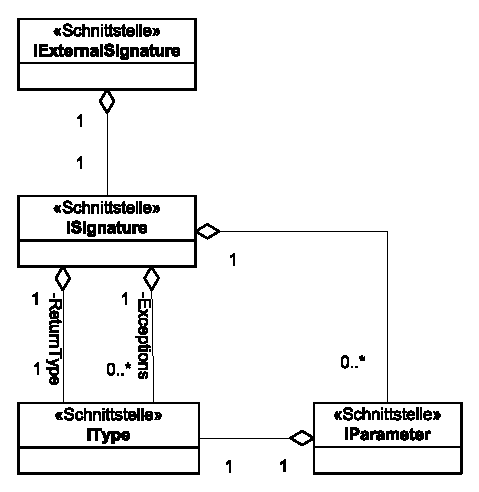
\includegraphics{pics/signatures.eps}
	\caption{Signaturen}
	\label{fig:signatures}
\end{figure}

There is nothing unusual about this. A signature is characterised by a return type, an identifier, an ordered list of parameters and an unordered list of exceptions (note that exceptions are not part of the standard interface/signature model in .NET). Additionally, as noted in the introduction there are external signatures consisting out of a role and a signature (the association to the role can be seen in figure \ref{fig:classdiagramm}).

\subsection{Connections}

Connections are part of composite components and are used to connect roles of components. They are modelled as depicted in figure \ref{fig:connection}. 

\begin{figure}[htb]
	\centering
		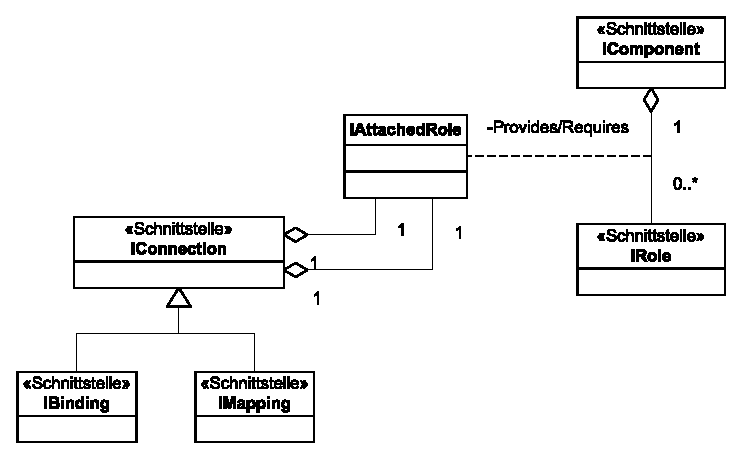
\includegraphics[scale=0.95]{pics/connection.eps}
	\caption{Connections, Mappings and Bindings}
	\label{fig:connection}
\end{figure}

There are two specializations of a connection: binding and mapping (see also figure \ref{fig:connections}). Bindings connect required roles to provided roles in order to fullfill the need for service. Mappings are only logical connections between the outer interfaces of a composite component and the inner ones. A connection always runs from a requiring role to a providing one (in the case of mappings this might sound a bit strange, but just imagine the outer interfaces having a mirror interface to the inside of a composite component). One important aspect of connections is, that it is assumed that a connection is valid with respect to the services required and provided, e.g., that every required service can be found exactly on the provides role. Renamings, parameter changes, overload resolving and the like is not done along a connection. If it is necessary to introduce such things one has to introduce an adaptor for these tasks.

\subsection{Full static structure}

The complete structure is depicted in figure \ref{fig:classdiagramm}.

\begin{figure}[htb]
	\centering
		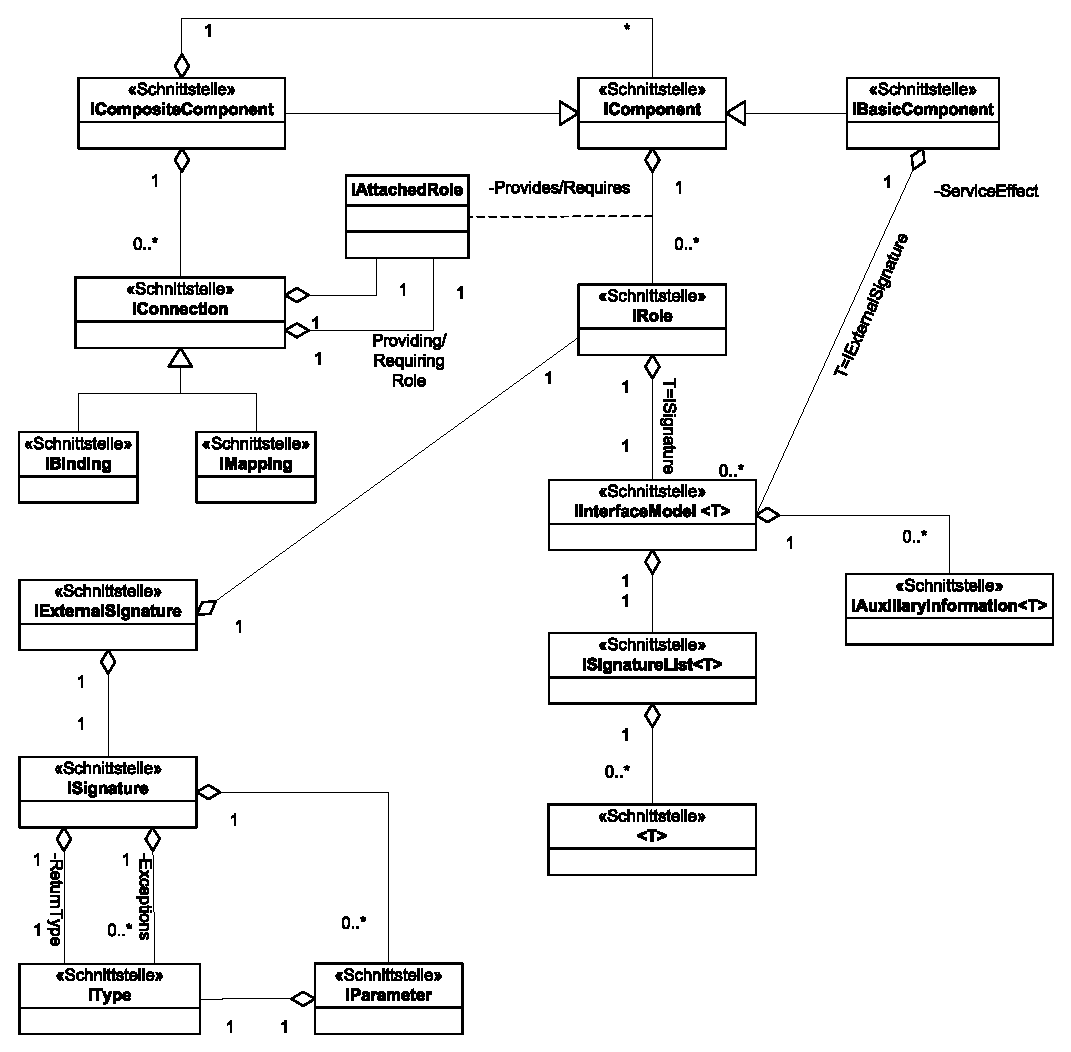
\includegraphics[scale=0.95]{pics/classdiagramm.eps}
	\caption{Full Class Diagramm of the Palladio Component Model}
	\label{fig:classdiagramm}
\end{figure}

\end{document}
